\documentclass[12pt, a4paper]{scrartcl}
\usepackage[utf8]{inputenc}
\usepackage{graphicx}
\usepackage{amsmath, amsthm, amssymb, textcomp}
\usepackage{setspace}
\usepackage{paralist}
\usepackage{graphicx}
\usepackage{caption}
\graphicspath{{WSK_im/}} %Graphic is in a folder named WSK_im in the currend directory
\usepackage{float}
\usepackage{authblk}
\renewcommand\Authfont{\fontsize{12}{14.4}\selectfont}
\title{Bayesian probability theory - Lesson 6}

\author{Wolfgang von der Linden}
\date{Transscript}

\begin{document}
\setlength{\parindent}{0pt}
\maketitle
\onehalfspacing
Welcome to unit six of the course on Bayesian probability theory. 
My name is Wolfgang von der Linden and I will enable you to help 
Captain Bayes and her crew in Bayesian deep reasoning.
This unit is dedicated to the central part of this course, namely \textbf{Bayes’ theorem}.

We will learn how to apply Bayes theorem to \textbf{solve inverse problems}
like to find a probability for having found treasure island,
we will learn how to assign probabilities in the Bayesian way using the
\textbf{principle of maximum entropy}
and we will learn how to \textbf{update probabilities} based on new information.\\

Now we come to the philosopher’s stone in probability theory: \textbf{Bayes’ Theorem}.
It turn noisy data and erroneous information into precious results: You can
use it
if you want to \textit{infer the parameters of your model from measured data},
if you want to \textit{quantify the uncertainty of the parameters},
if you want to \textit[{access the validity of your model},
if you want to \textit{access the validity of certain hypotheses}.\\

Let A and B be two arbitrary propositions, then the product rule tells us. \[P(A,B|I)=P(A|B,I)P(B|I\]
Alternatively since $A\hat B=B\hat A$ we find \[P(B,A|I)=P(B|A,I)P(A|I)\]
So the right hand sites have to be equal, leading to \textbf{Bayes’ Theorem}.
\begin{equation*}\boxed{P(A|B,I)=\frac{P(B|A,I)P(A|I)}{P(B|I)}
}\end{equation*}\\
Let’s assume A is the object of interest, e.g, parameters of a model and B
are the measured data. In this context, the terms in Bayes’ theorem have
the following names and meanings:
The term on the left hand site ($P(A|B,I)$) is the \textbf{posterior probability},
it is the probability for the quantity of interest \textit{after} adding new
information, therefore posterior.
The counterpart $P(A|I)$ is the \textbf{prior probability}. It encodes our
knowledge \textit{prior to adding the new information} into the inference.
The meaning of prior and posterior is not necessarily to be understood
in a temporal sense, but only in the order in which we consider the
information in the inference process.
The term $P(B|A,I)$
 is the so-called \textbf{likelihood}. You may think to
yourself, that’s a probability after all, why isn’t it called like that. And you
are partly right: it is a probability for B, but we are interested in A.
And in terms of A it is not a probability.
But in many cases, however, if the likelihood increases by varying A
that also means that A is more likely.
It is good to make this distinction in the naming of the terms, because
the\textit{ rules of probability do not apply to the likelihood as far as A is
concerned}\\
If you disregard this inequality you could end up in prison!
\textit{``Fun''fact: Disregarding this inequality let to catastrophically wrong judgments in a court case. }%%what
We finally arrive at the term in the denominator $P(B|I)$ of Bayes’ theorem.
It guarantees the normalization of the posterior and is called \textbf{normalization constant}. 
In a deeper sense it is the \textit{data evidence}.
Let’s assume A is part of a set of \textit{complete
and exclusive propositions}. (Do you still know what that means?) Then
the denominator has a simple form:
\[P(B|I)=\sum_nP(B|A_n,I)P(A_n|I)\]
In the following we will omit the background information $I$.\\

The first and most simple application of Bayes’ theorem is given, if the set
only consists of one proposition A and its complement A. I leave it up to
you so solve the following question:\\

\textit{Given a rapid antigen test, that gave the result positive or negative,
what is the probability to have the virus or not to have the virus?}
%6_1
 \begin{figure}[H]
	\centering
	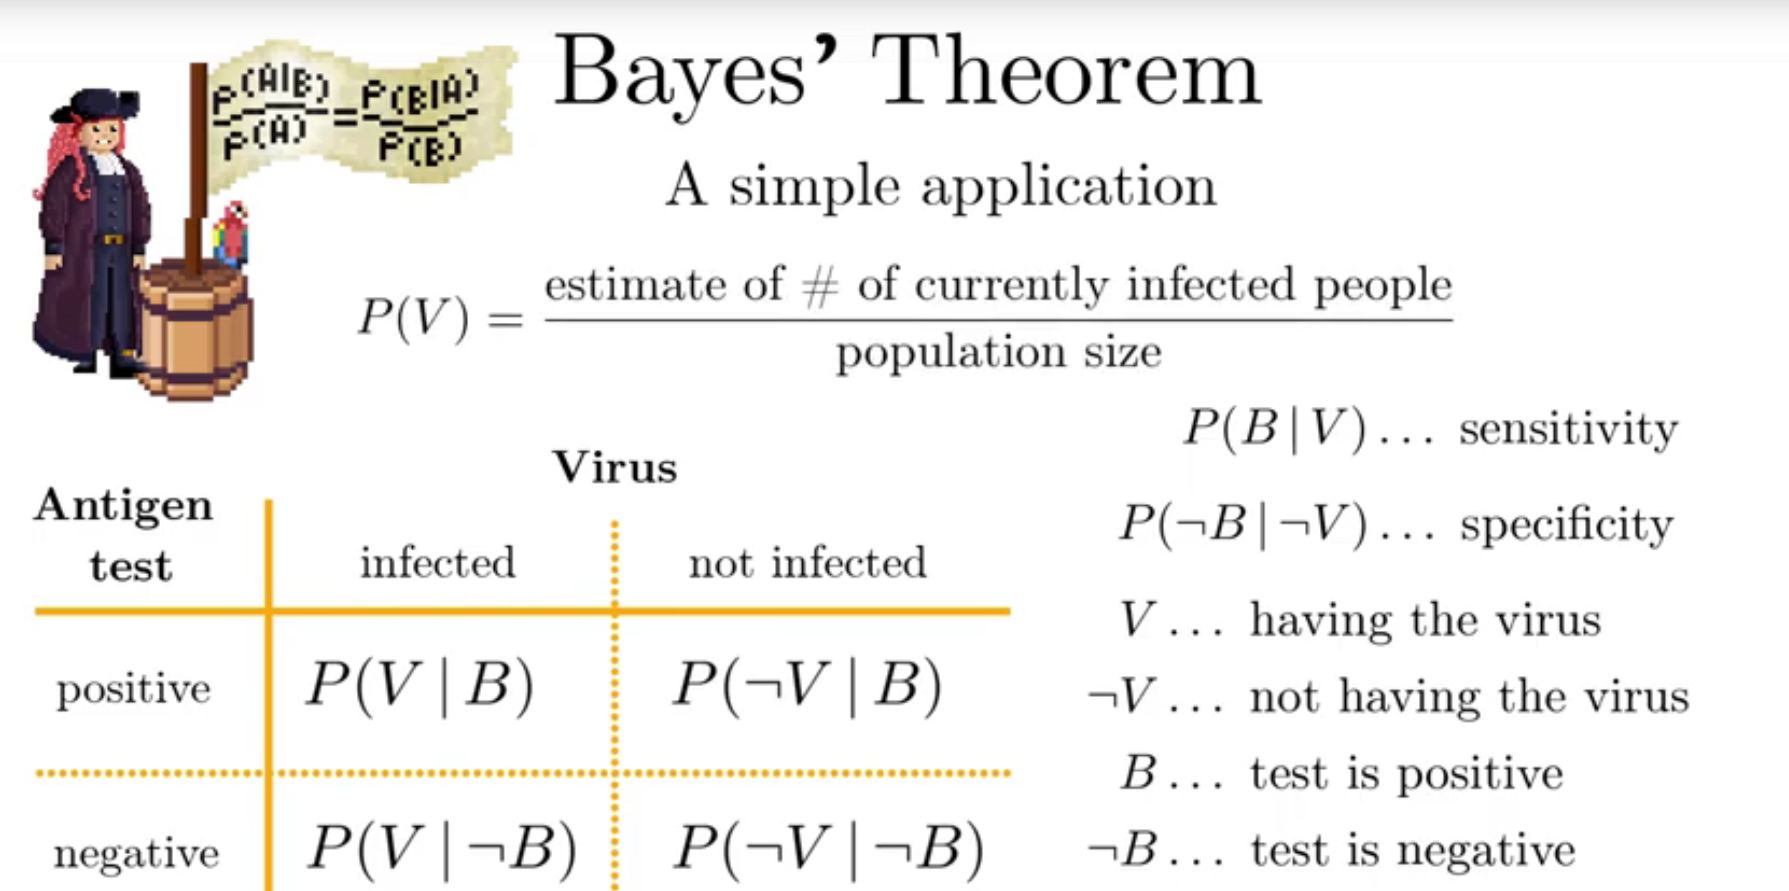
\includegraphics[width=0.75\textwidth]{6_1.png}
\end{figure}
To answer this question, we need the \textit{sensitivity} $P(B|V)$ and the \textit{specificity} $P(\not B|\not V)$ of the test
In addition we need the \textit{prior probability} $P(V)$ for a person to have the virus
without additional information.\\

Now we want to apply Bayes’ theorem to the treasure island problem. Captain Bayes 
correctly pointed out that the draftsman of the map wanted to
give us a hint with the name ”Inverse sea”. Because this is indeed an \textbf{in-
verse problem}. And of course the letter of her brother Thomas Bayes has
the solution to it.
Why inverse? Because, the likelihood corresponds in a sense to the forward
problem. If we know the island, we also know the percentage of frog-fish $Q$
and then the likelihood of catching K frogfish is straight \textbf{forwardly}
computed. It is given by the probability for K frogfish in a catch of size N
and as such it is a binomial distribution. \[P(K|Q,N)={N\choose K}Q^K(1-Q)^{N-K}\]
But we are interested in the inverse probability: \textit{The probability that this is
a particular island given the number K frogfish in a catch of a 100 fish in
total} P(treasure island $|K, 100$).\\

We introduce the propositions concerning the island $I_i$ where i= 1 stands for
treasure island, i=2 for paradox island and i=3, as conjectured by Pascal,
for an unknown island. The desired probability is given by Thomas Bayes’
theorem. \[P(I_i|K,N)=\frac{P(K,I_i,N)P(I_i|N)}{Z}\]
Here the second factor in the numerator is the prior probability, the one without the result of the fishing, so $P(I_i|N)=P(I_i)$.
Let’s assume that the prior probability for the unknown island is $\alpha$ and very
small, while the probability for treasure and paradox island are the same (namely $\frac{1-\alpha}{2}$).\\%

Then the likelihood $P(K|I_i,N)$ for the two known islands is binomial
where $Q_i$ is the corresponding frogfish ratio,
$Q_1 = 0.1$ for treasure island and $Q_2 = 0.2$ for paradox island.
The remaining unknown probability is the likelihood for the third island.
If the island is unknown, then the frog-fish ratio is also unknown, and thus
this probability is \textit{independent of K} $P(KYI_3,N)=\frac{1}{N+1}\Theta(0\leq K\leq N)$ (this function is simpy a constant function between 0 and N)
Finally, the normalization has the form given before for complete and exclusive events.\[Z=\sum_iP(K|I_i,N)P(I_i)\]

By now we have everything we need to apply it to the Bayesian adventure
where they counted or - in the terms of Captain Venn - measured 14 frogfish
in a catch of 100 fish.
To begin with, we assume there are just the two islands mentioned in the
treasure-map. Then alpha is equal to zero and we obtain that the posterior probability for
treasure island is 0.605. Therefore, the crew will decide that the island 
they found is almost certainly treasure island.
But what if we allow for the third alternative and assume, since we don’t
know any better, that all three islands have the same probability one third, so $P(I_i)=\frac 13$.
Then we obtain completely different posterior probabilities.\\%6_2
 \begin{figure}[H]
	\centering
	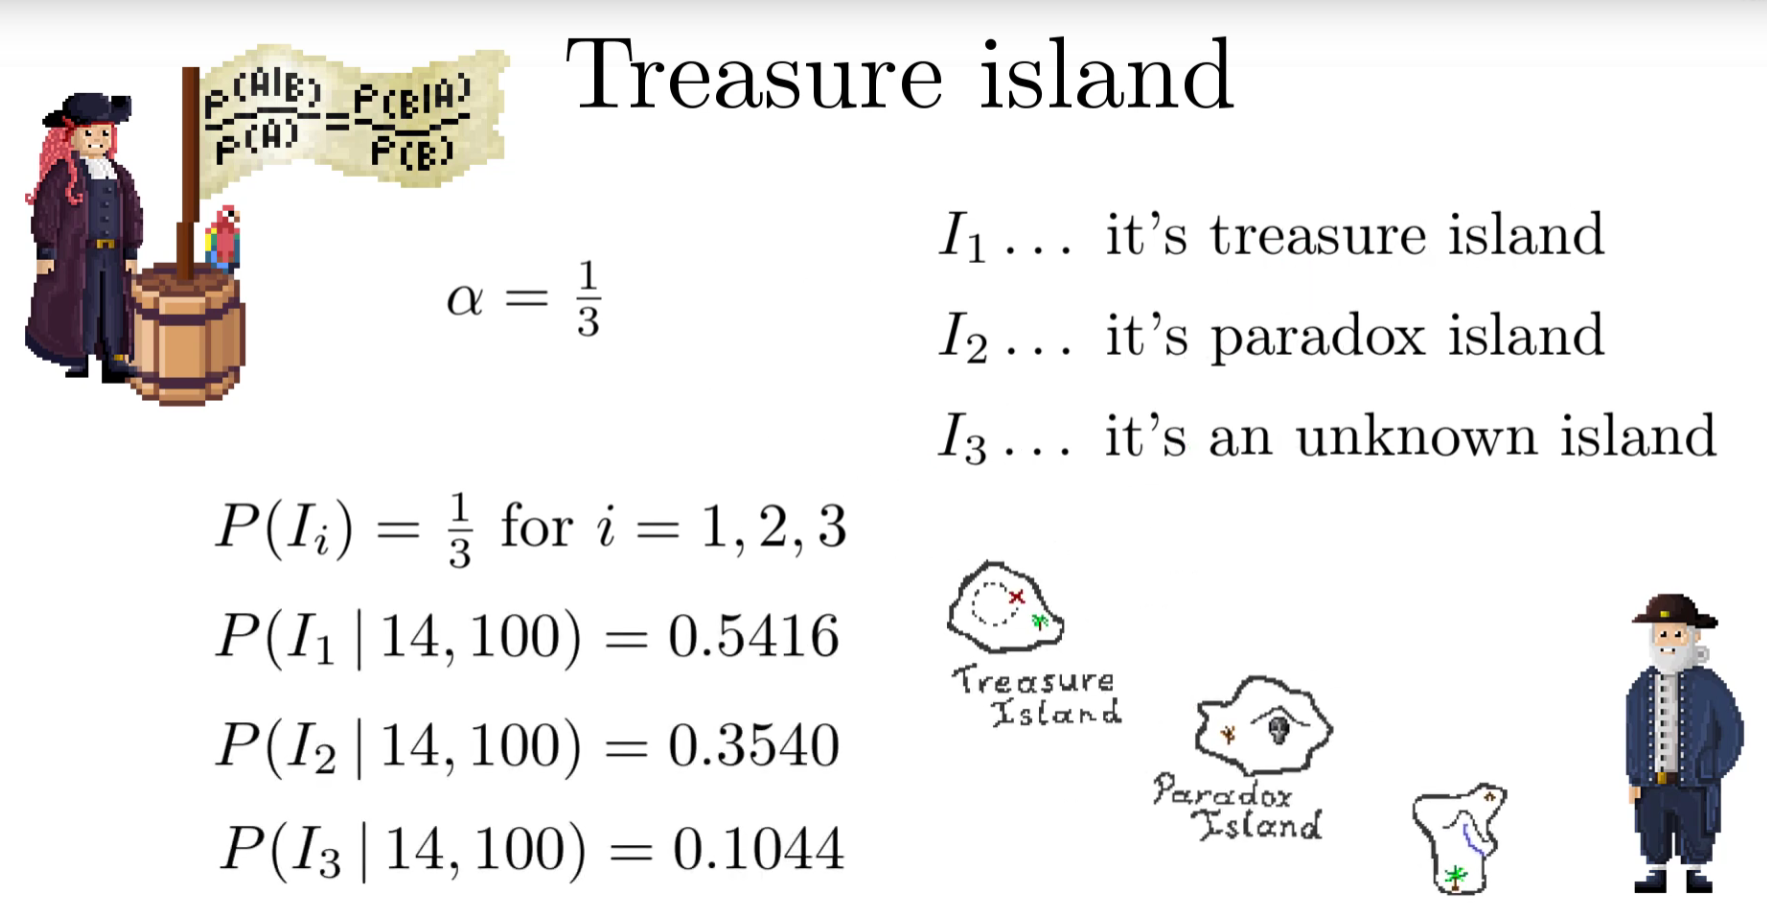
\includegraphics[width=0.75\textwidth]{6_2.png}
\end{figure}


When Captain Bayes visited Claire’s pottery store she was wondering:
”It would be an intriguing question whether you can guess
this distribution just from the mean starfish ratings?”
\textit{Guessing a distribution just from its mean value} is a very general question, it
concerns the assignment of prior probabilities. For the task of assigning
prior probabilities we so far only know the principle of indifference based on
symmetry or indifferent properties leading to a \textbf{uniform distribution}.
We will now learn how to combine those techniques, so how to use additional
so-called \textbf{testable information}, such as the mean starfish-rating, which will
lead us to a non-uniform distribution.\\

The general approach is the so-called \textbf{maximum entropy method}. The main
idea is to evaluate \textbf{Shannon’s entropy} S for a probability distribution.%
\begin{equation*}\boxed{S(!)=-\sum_{i=1}^MQ_i\ln(Q_i)
}\end{equation*}\\
It is a measure for the uncertainty, encoded in the probability distribution.
Before we show that this statement is plausible guided by a simple example,
let us discuss some details of the entropy.
The individuals summands $S(Q_i)$ are \textit{greater or equal to zero},
and they are only zero in the case of \textbf{certainty}, which means the corresponding event
will definitely happen (Q = 1) or will definitely never happen
(Q = 0) .
In between the entropy looks like an inverse parabola.\\%6_3
 \begin{figure}[H]
	\centering
	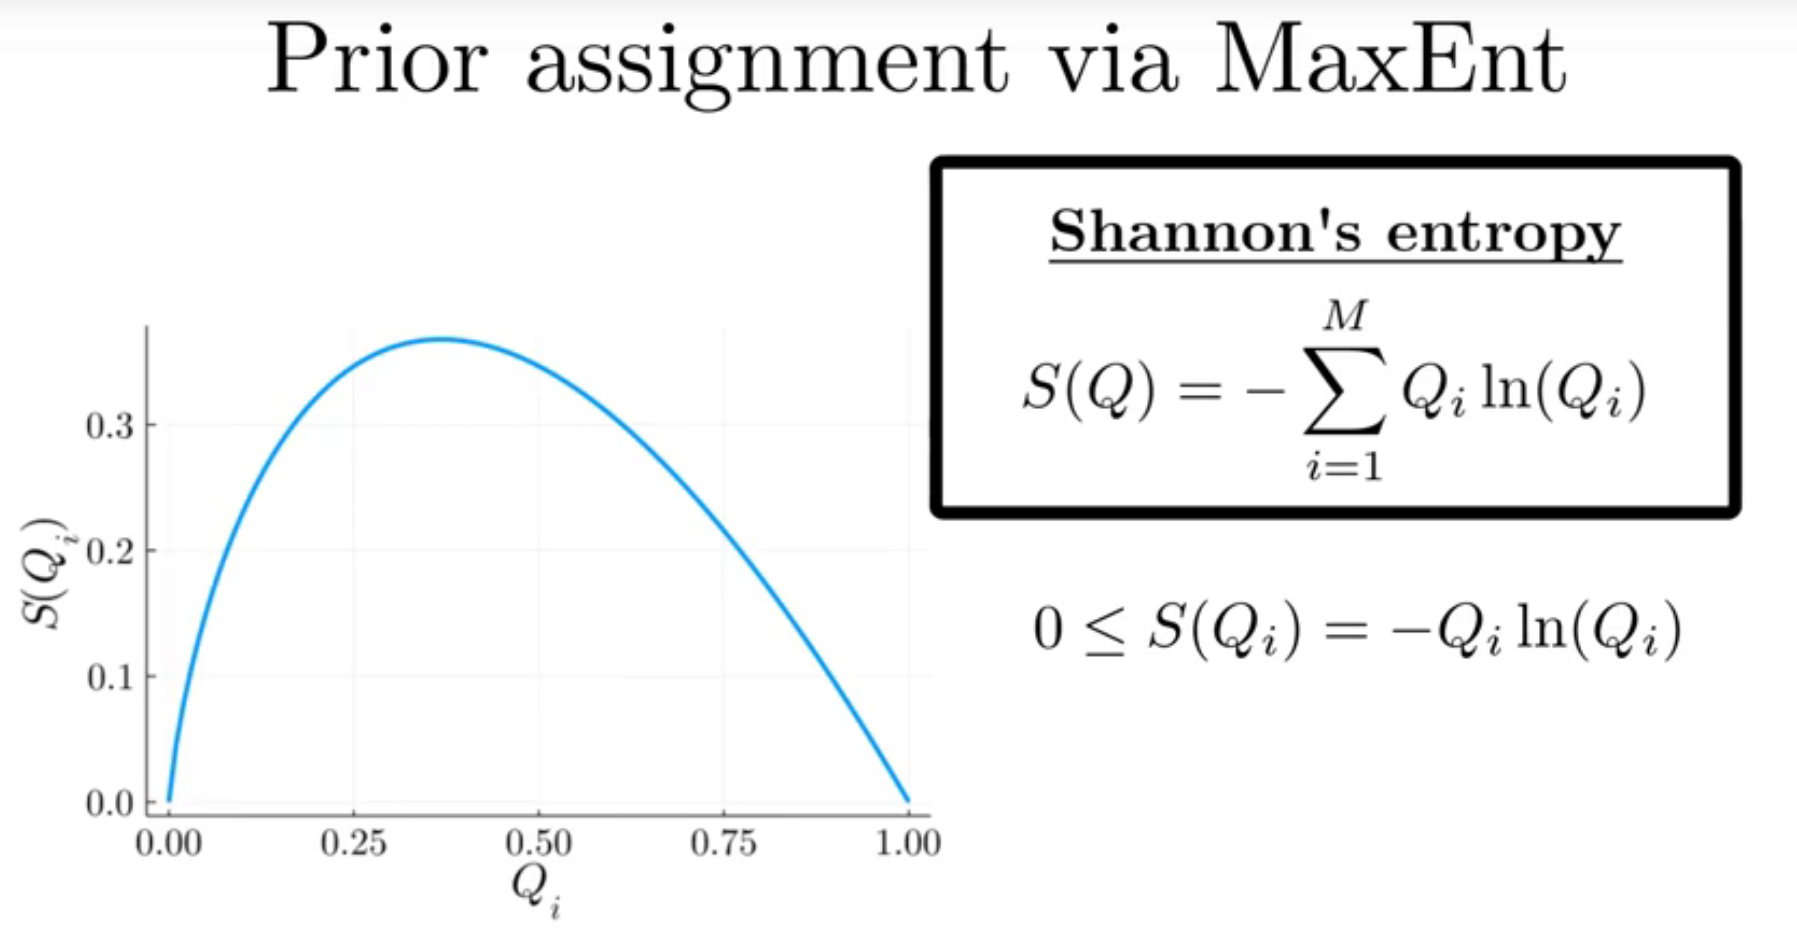
\includegraphics[width=0.75\textwidth]{6_3.png}
\end{figure}

The total Shannon entropy is zero if the \textit{entire probability mass is concen-
trated at a single index}, so Q=(0,0,0..,0,1,0,...0,0).
Zero entropy means zero uncertainty, or rather we are certain about the
outcome of the corresponding event. The most uncertain or vague probability
distribution is the one that \textit{maximizes the entropy} but still \textit{fulfils the
normalization constraint}.
\begin{equation*}\boxed{\Phi_0=\sum_{i=1}^MQ_i-1\stackrel{!}{=}0
}\end{equation*}\\
The most uncertain distribution fulfilling that constraint will be proven soon
to be the uniform distribution.\\
\begin{equation*}\boxed{Q_i^{uni}=\frac 1M
}\end{equation*}\\
This is reasonable, as
the entropy does not make any difference between the individual terms, so the principle of indifference still holds.
The \textbf{entropy} for a uniform distribution is the logarithm of the number of
outcomes.\\

\begin{equation*}\boxed{S(Q^{uni})=-M\frac 1M \ln\left(\frac 1M\right)=\ln(M)
}\end{equation*}\\

Let’s consider some simple examples of distributions which all yield a
mean value of 3:\\ %6_4
 \begin{figure}[H]
	\centering
	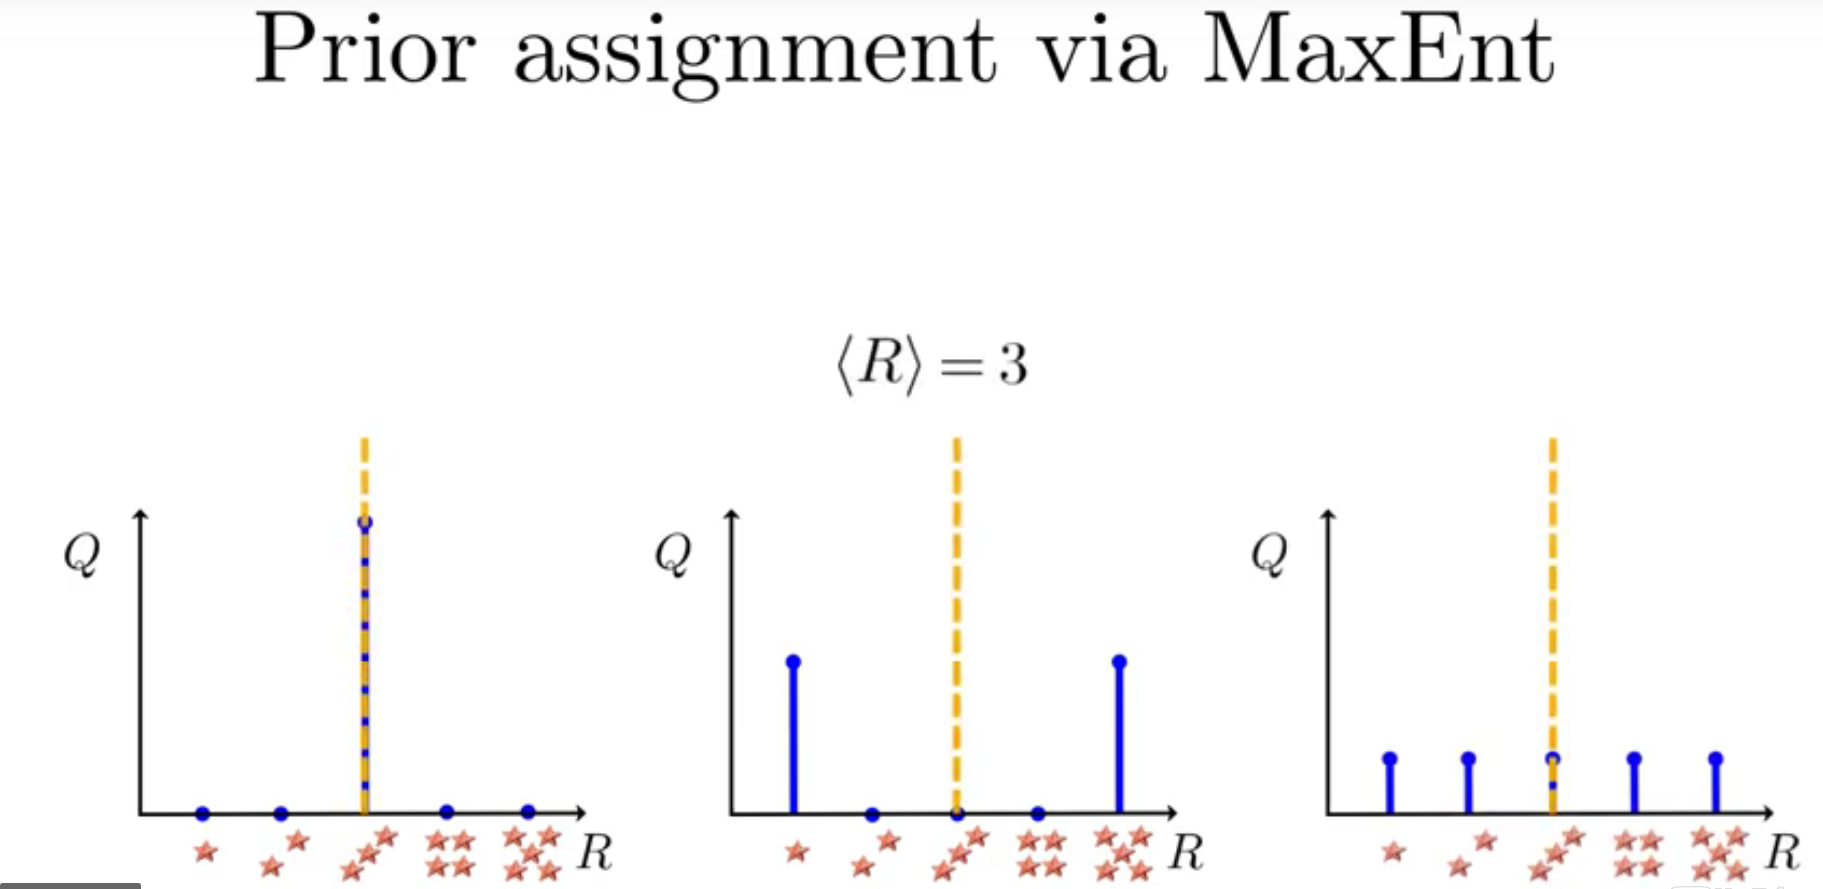
\includegraphics[width=0.75\textwidth]{6_4.png}
\end{figure}

One possibility for the intrinsic starfish-rating could be a distribution
that encodes \textbf{certainty}, because it would always predict to obtain 3 starfish.
The corresponding \textit{entropy is 0}, as outlined before.

Next we consider a distribution, which is a little more insecure as it predicts to see the rating values 1 and 5 stars
with \textbf{equal probability}. The corresponding \textit{entropy is ln(2)} which is
obviously greater than 0.\\

Finally we consider the \textbf{uniform distribution}. This is the least committed distribution and it has, as we know already, the greatest \textit{entropy ln(5)}.
So, if we know only the mean being 3 of a normalized probability distribution
in the case of the starfish-rating, then the uniform distribution is the best
choice. It fullfills the constraint but it \textit{adds no extra information}.
Any other distribution favours some starfish-rating values over others, which
is not supported by the mean value of 3.
If we prefer a distribution that has a lower entropy than the maximum possible 
given the constraints, then there has to be \textbf{additional information} to support it.
By now, you should be able to guess how to proceed, if additional so-called
testable information, like the mean starfish-rating, is given.\\%6_5
 \begin{figure}[H]
	\centering
	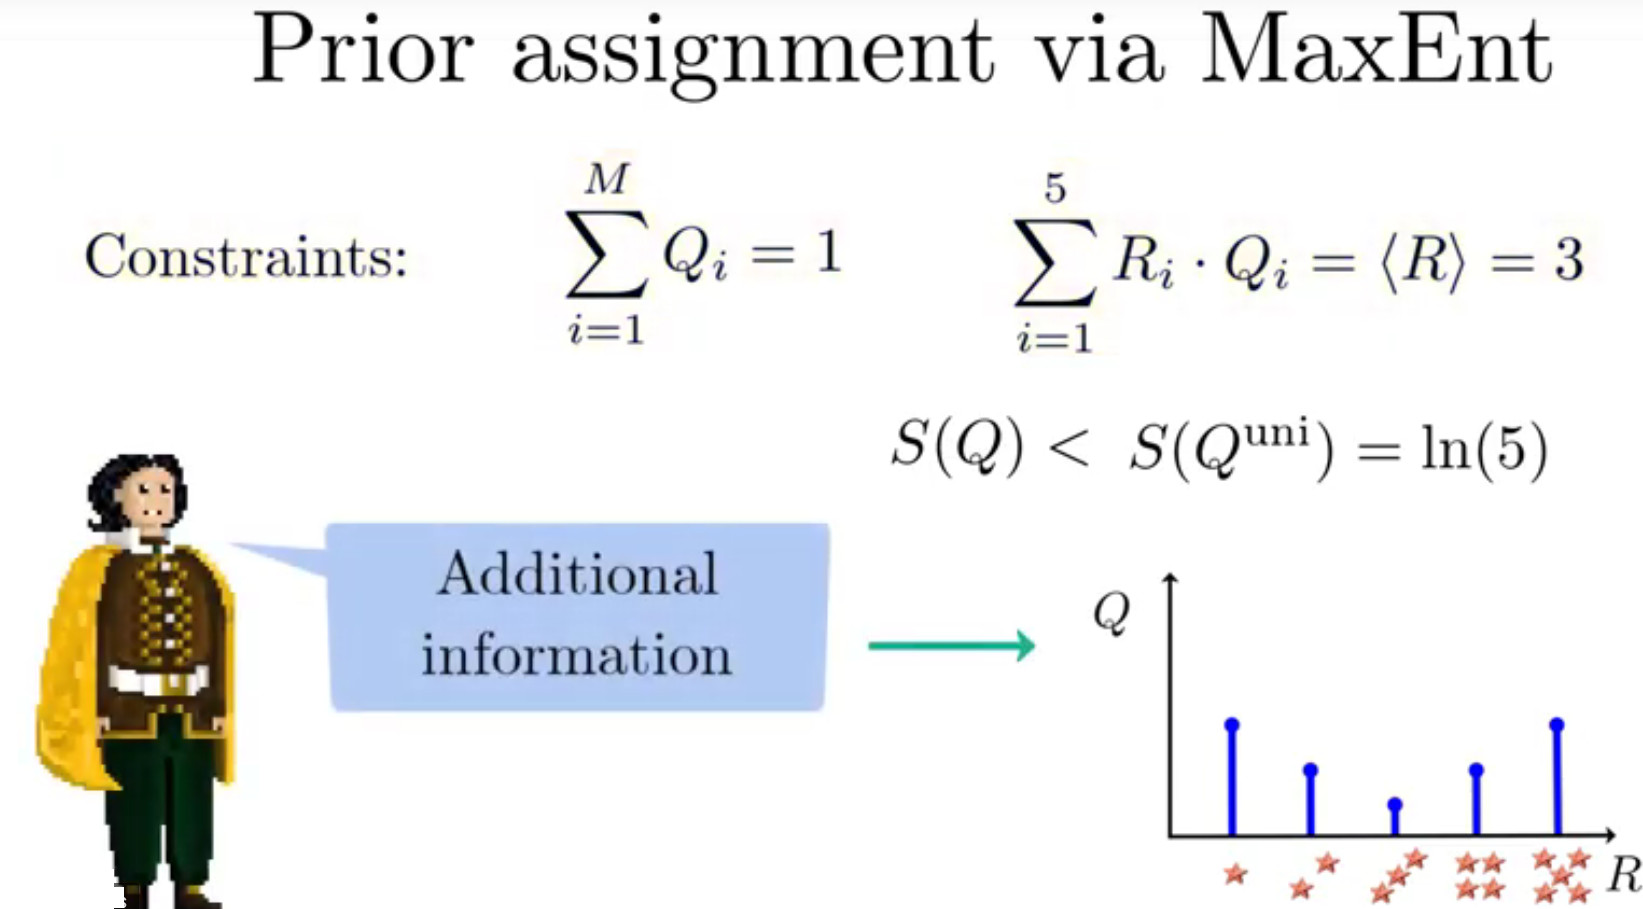
\includegraphics[width=0.75\textwidth]{6_5.png}
\end{figure}

I am sure you got it right. The \textit{entropy has to be maximized fulfilling
all the constraints} including normalization. For the sake of clarity we
will only use one constraint \[\Phi_i=\sum_{i=1}^MR_iQ_i-\mu\stackrel{!}{=}0\], so a fixed mean value $\mu$ in addition to the normalization. 
Maximizing the entropy under those constraints leads to probabilities
that are consistent with the constraints but otherwise as \textbf{uninformative} or
\textbf{uncommitted} as possible. If you draw conclusions based on the maximum
entropy probability distribution, the \textit{deviation to the true result is thereby
minimized on average}.
Constrained maximization can be achieved most elegantly by the method of
\textbf{Lagrange multipliers}. We define the so-called \textbf{Lagrangian}.\\%6_6
 \begin{figure}[H]
	\centering
	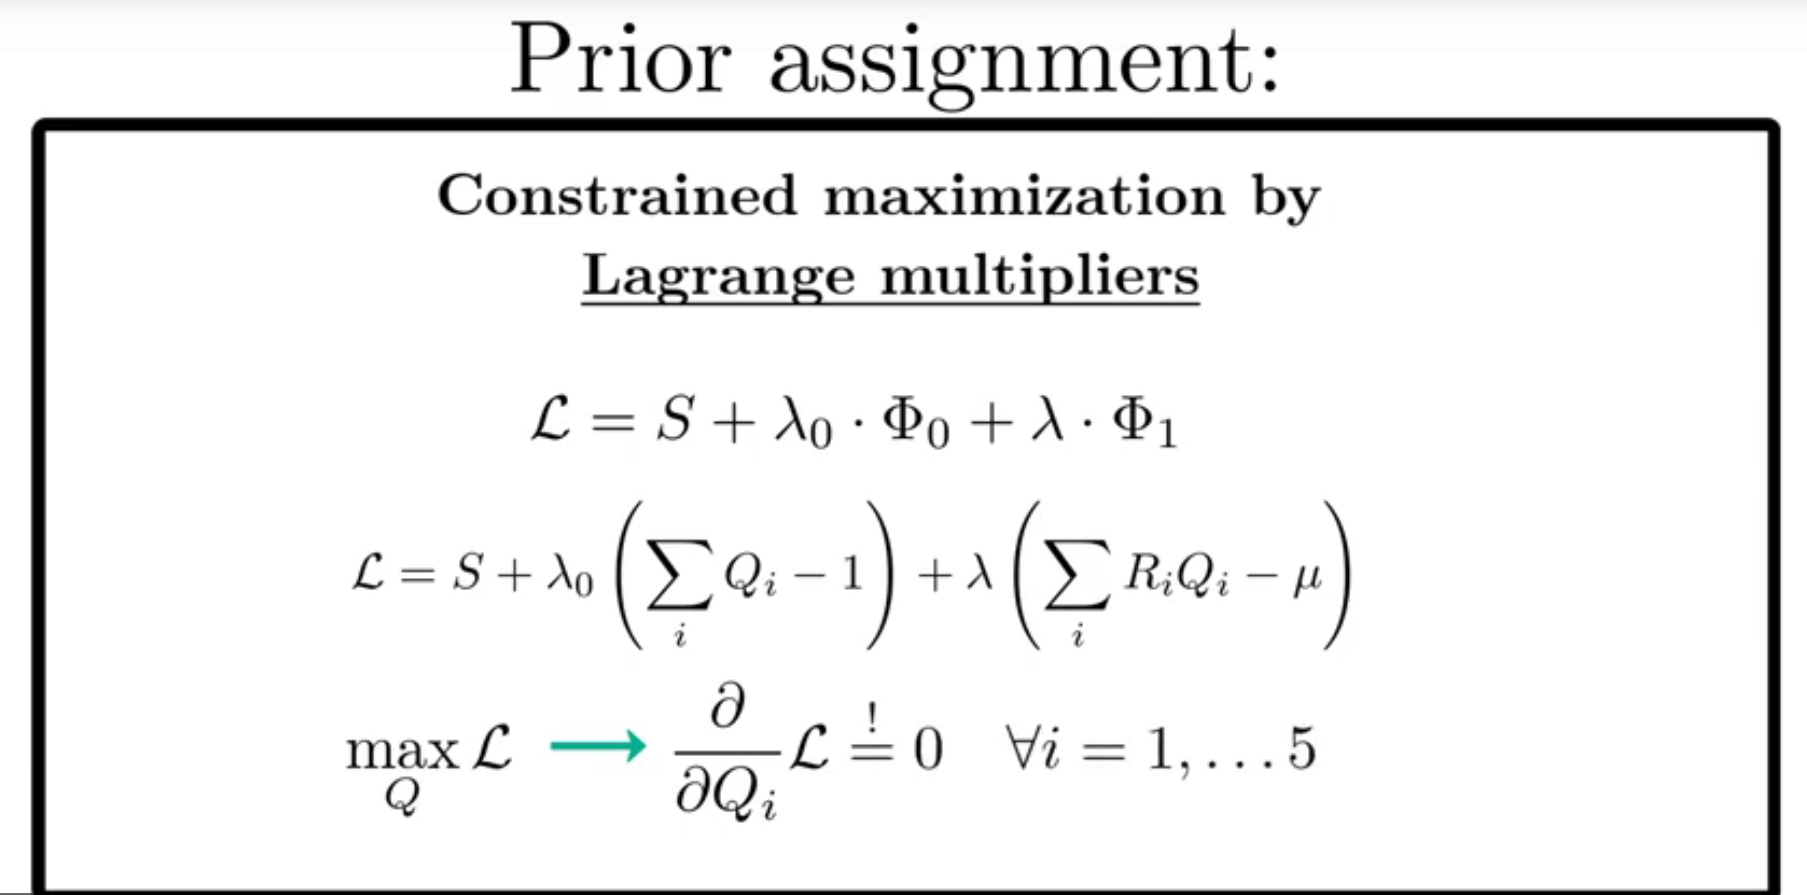
\includegraphics[width=0.75\textwidth]{6_6.png}
\end{figure}

The maximization condition is that the \textit{derivative with respect to the probabilities vanishes}.
The derivative can be computed easily and we obtain an exponential expression for the probabilities.\\

\begin{equation*}\boxed{Q_i=e^{-1+\lambda_0}e^{\lambda R_i}
}\end{equation*}\\

The normalization Z follows readily: $Z=\sum_ie^{\lambda R_i}$
The second Lagrange parameter $\lambda$ follows from the second constraint.
%6_7
 \begin{figure}[H]
	\centering
	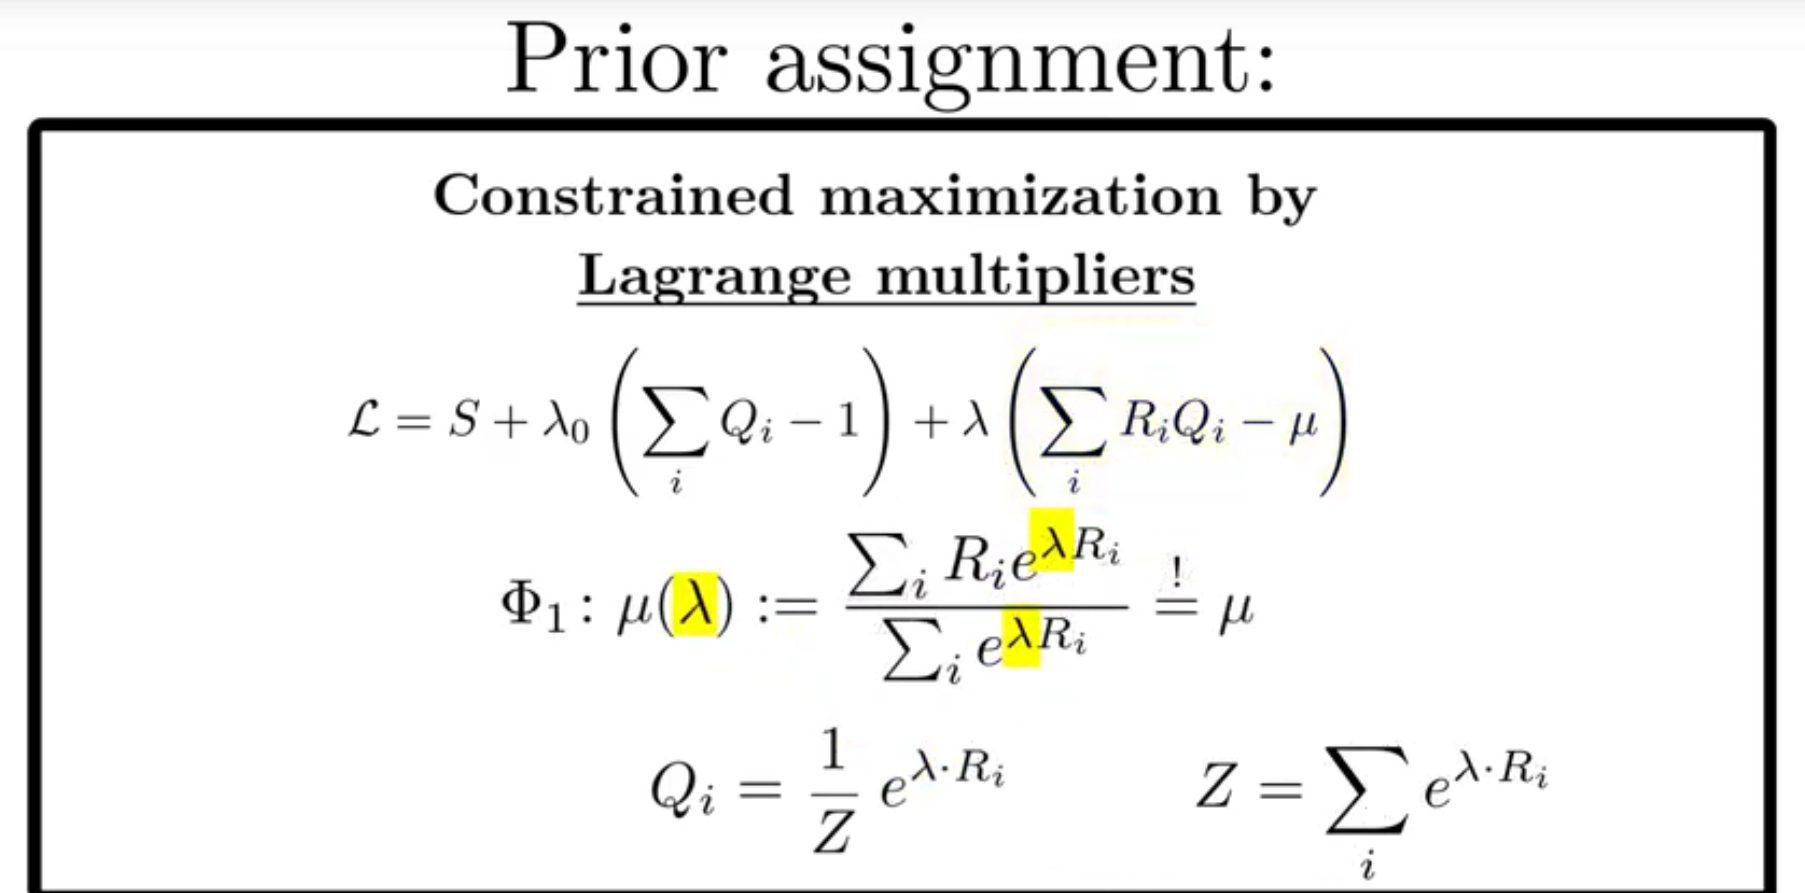
\includegraphics[width=0.75\textwidth]{6_7.png}
\end{figure}
We cannot solve that in a closed form but the result can be obtained easily
by numerical means.
The behaviour of $\mu(\lambda)$ can be estimated qualitatively. In the limit $\lambda\rightarrow -\infty$
only the R=1 term survives resulting in $\mu = 1$ and in the opposite
case$\lambda \rightarrow \infty$ only R = 5 survives, leading to $\mu=5$. In between, the
function increases monotonically, as you can see in the figure. %6_8
 \begin{figure}[H]
	\centering
	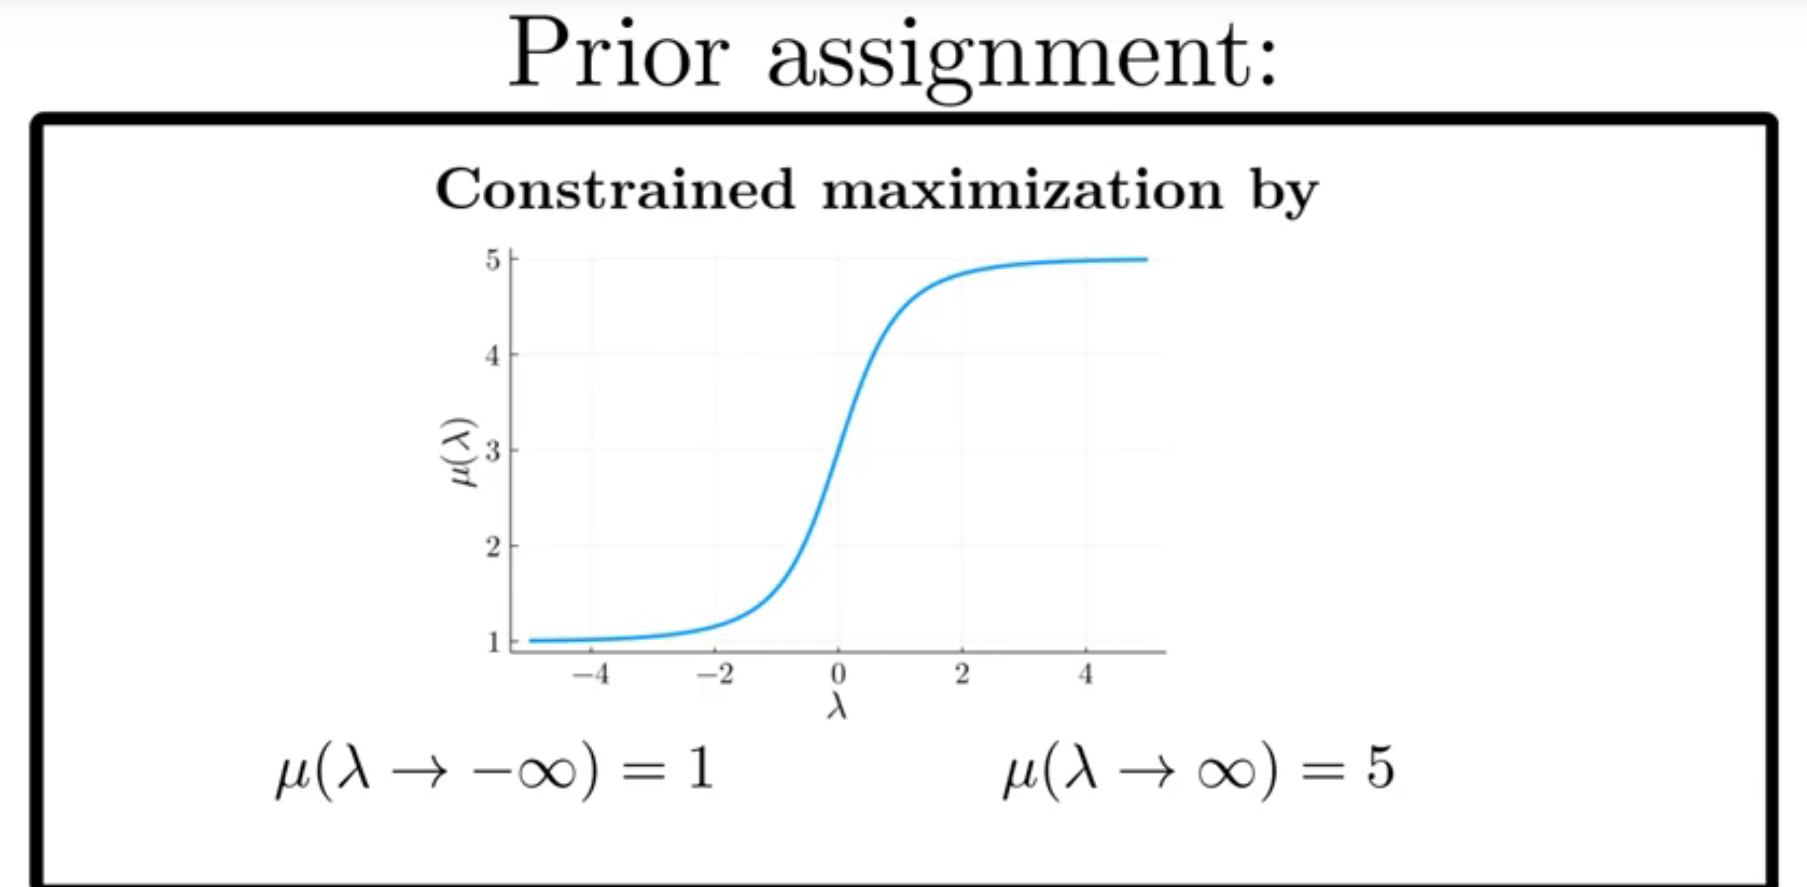
\includegraphics[width=0.75\textwidth]{6_8.png}
\end{figure}
Since the curve
increases monotonically, for each mean $\mu$ there exists a unique solution for
the Lagrange parameter $\lambda=\mu^{-1}(\lambda)$. For $\mu =4.5 \Rightarrow \lambda=1.07$, that leads to rating probabilities \[Q^{(\mu=4.5)}=(0.01,0.03,0.07,0.23,0.66)\]

For the numerical determination of the Lagrange-parameter $\lambda$
the \textbf{Newton-Raphson} method is ideally suited in this case. The result depends on the
intrinsic or true mean $\mu=\langle R\rangle$ and reads\\%%

\begin{equation*}\boxed{P(R_i|\mu)=Q_i^{(\mu)}=\frac{e^{\lambda(\mu)R_i}}{\sum_{i=1}^5e^{\lambda(\mu)R_i}}
}\end{equation*}\\

\textit{You will find a Pluto note book, where you can experiment with different
mean starfish-ratings and obtain the corresponding rating probabilities.}\\

Captain Bayes found the starfish-rating interesting, but slightly confusing,
as the number of votes was different for the various items. We will discuss
the \textbf{reliability} of the voting in two steps, first by a sort of a statistical experiment and
then in the correct Bayesian framework.\\%6_9
 \begin{figure}[H]
	\centering
	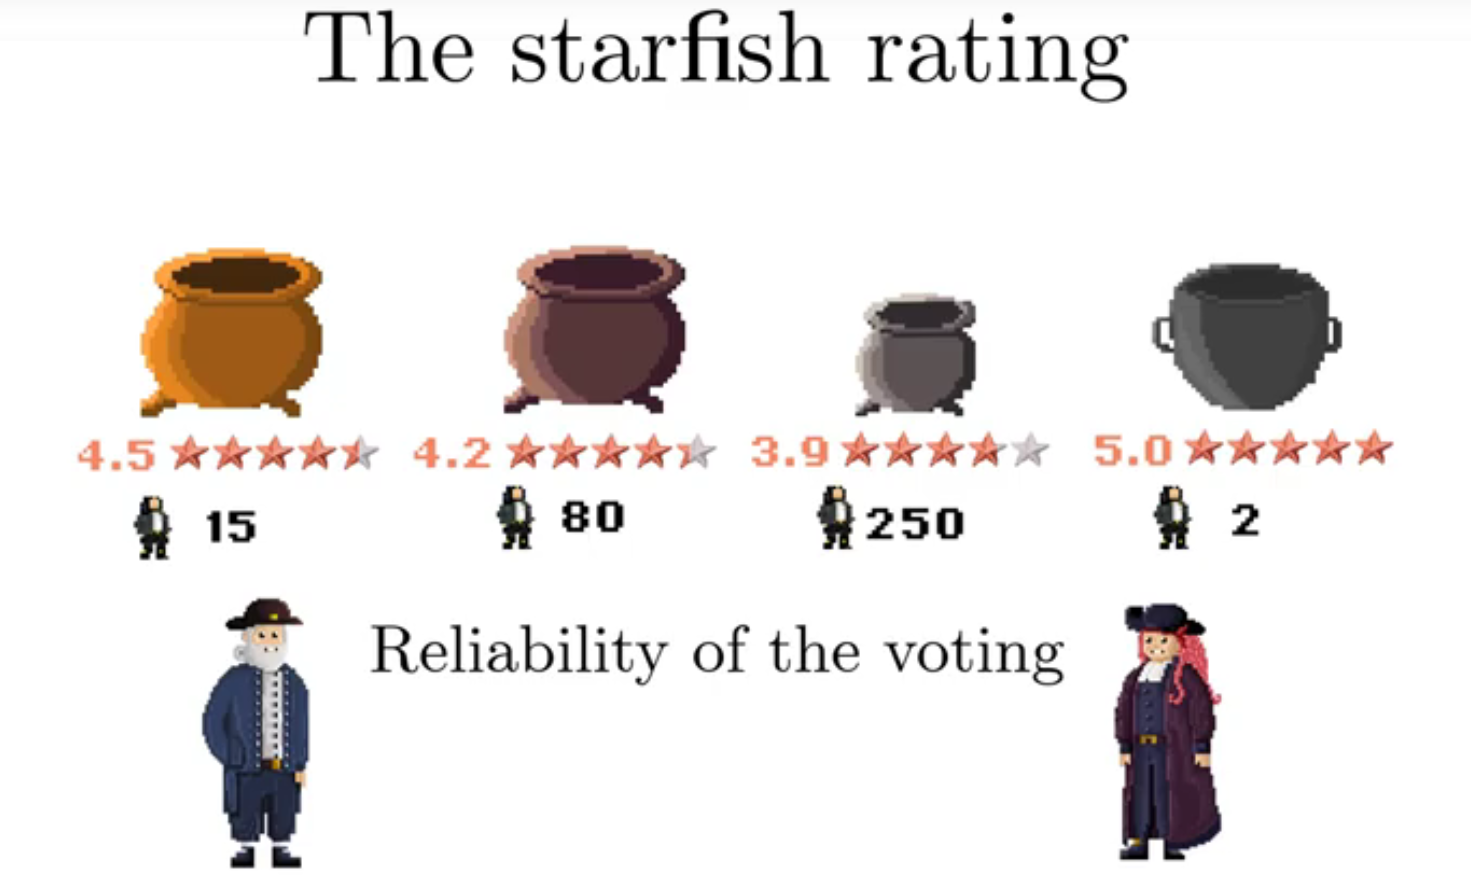
\includegraphics[width=0.75\textwidth]{6_9.png}
\end{figure}

Since we can’t try all four pots, we want to find out how good the pots really are
by a statistical experiment.
Take the measured ratings and think of how our own vote would be and how
it would change the overall rating.
For simplicity, let’s assume that starfish ratings are binary outcomes, which means we only have
\textit{”like”} or \textit{”dislike.”} So to describe the tin pot rating of 3.9 out of 5 starfish
with 250 votes with binary votes we have 195 likes and 55 dislikes. Let’s
assume Laplace has \textit{no preference}, so his prior prejudice is 50\% \textit{like} and 50\%
\textit{dislike}. Adding his own rating as one proportional vote leads to 195.5 likes
and 55.5 dislikes and a new rating of 3.89 starfish - so a very modest reduction.\\

For the iron vessel with 5 out of 5 starfish and two votes only, the situation is
different. Adding Laplace’s own reasoning leads to 4.2 starfish - so a strong
reduction that makes the other pots more likely to be a good choice, which
is plausible because you wouldn’t rely on an opinion of just two strangers.
Now this technique can be adopted in two ways. First, Laplace might have
concerns about the pots that are similar to the broken one, say the iron and
the tin pot, because they have similar colors to the old pot, so he might
change his mind and give only 0.3 likes to the tin and iron pot, for example.
Second, he could give \textit{more weight to his opinion} by contributing his opinion
as 2 or more votes rather than as a single vote.\\
\textit{There is a Pluto notebook waiting for you, where you can vary your own
opinion and appropriate weightings, and also explore how a prize can change
your personal decision!}\\


The historical Laplace had asked himself how likely it was that the sun would
rise again the next day, based on an estimated number of days it had risen
before. This is nowadays called the \textbf{Laplace law of succession}.
For the starfish rating the corresponding question would be: \textit{What is the
probability that the next vote will be R starfish, given the earlier votes.} This
is a nice exercise in Bayesian probability theory. \textit{Some details will be given
in the supplementary material.}\\


Now we turn to the correct \textbf{Bayesian approach} for the starfish rating. We
are interested in the probability for the \textbf{true/intrinsic rating} $P(\mu|\bar{R},N)$ , given the \textit{mean rating} $\bar{R}$ and the the \textit{number
of votes} $N$. The true rating is what you would get with an \textit{infinite number of votes}.\\

The first step is to invoke Bayes’ theorem to \textit{express the posterior in terms of likelihood and prior}.
\[P(\mu|\bar{R},N)\propto P(\bar{R}|\mu,N)P(\mu)\]
To be able to
compute the likelihood we need the \textit{individual ratings $R_i$ of all N voters},
which we introduce via the \textbf{marginalization rule}.
\[P(\bar{R}|\mu,N)=\sum_RP(\bar{R}|R,N)P(R)\]
 Here we used the fact that the individual votes are \textit{uncorrelated}, so not depending on $\mu$
The factors in the product are nothing but the rating probability we derived
in the maximum entropy section.\\%6_10
 \begin{figure}[H]
	\centering
	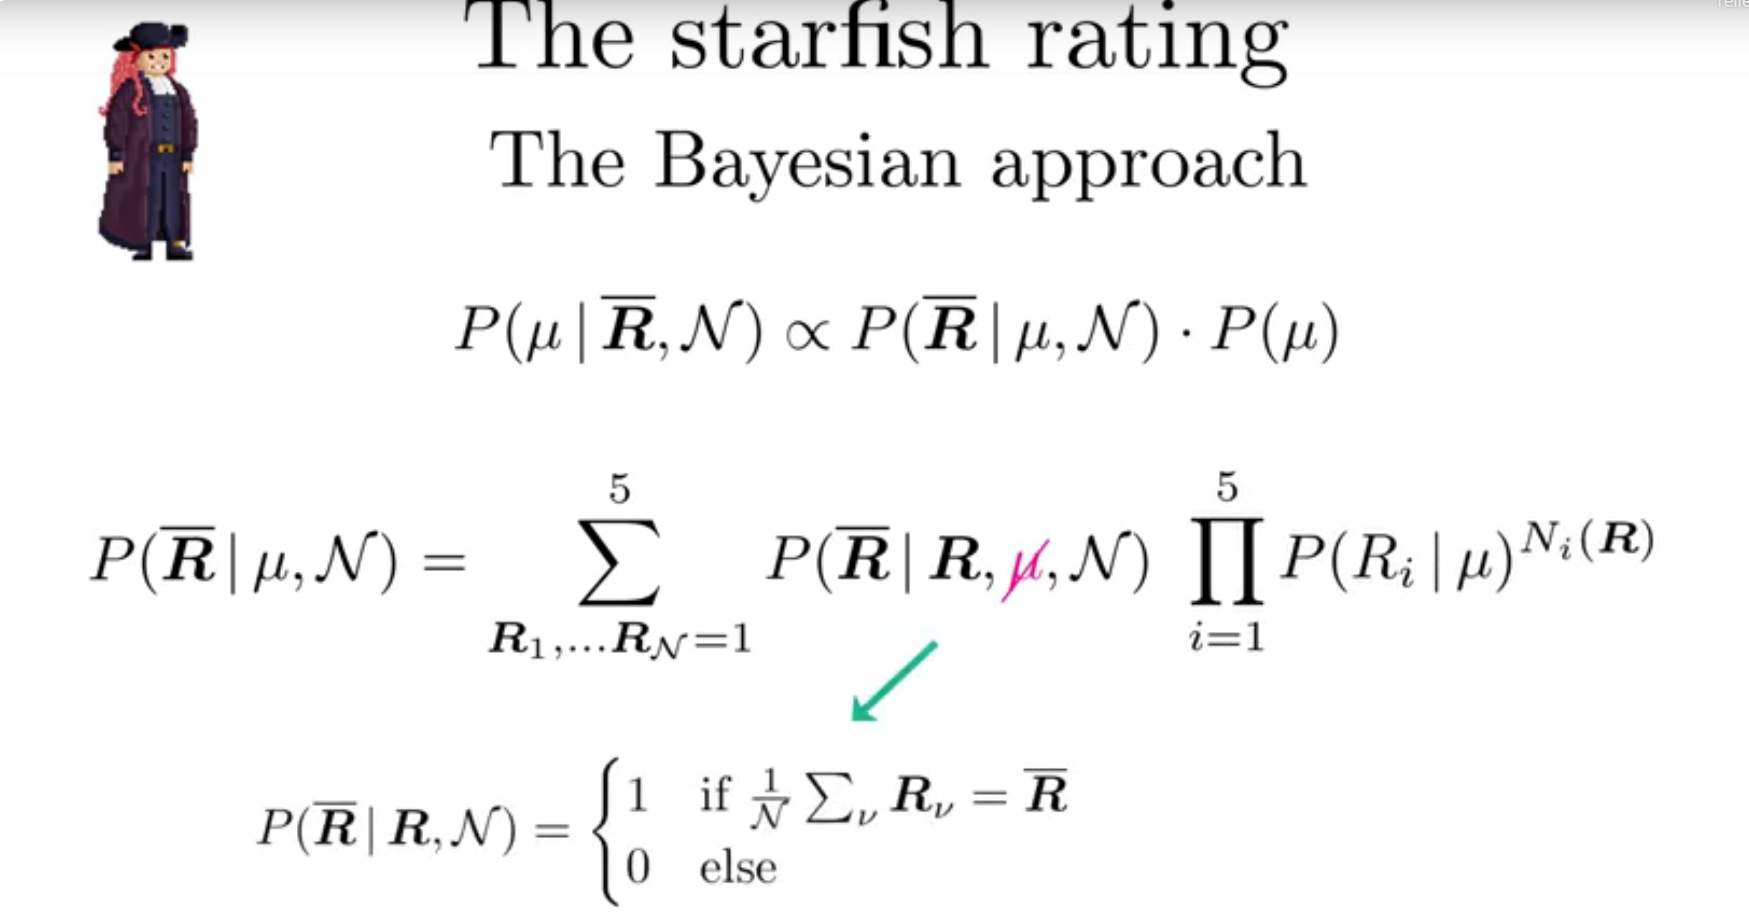
\includegraphics[width=0.75\textwidth]{6_10.png}
\end{figure}

That should be enough information for you to perform the remaining steps on
the Bayesian path yourself. But don’t be disappointed - the final expression
has to be evaluated numerically. That’s mostly the case in all real world
problems.\\%

The figures show the results for the copper pot and the iron vessel. %6_11
 \begin{figure}[H]
	\centering
	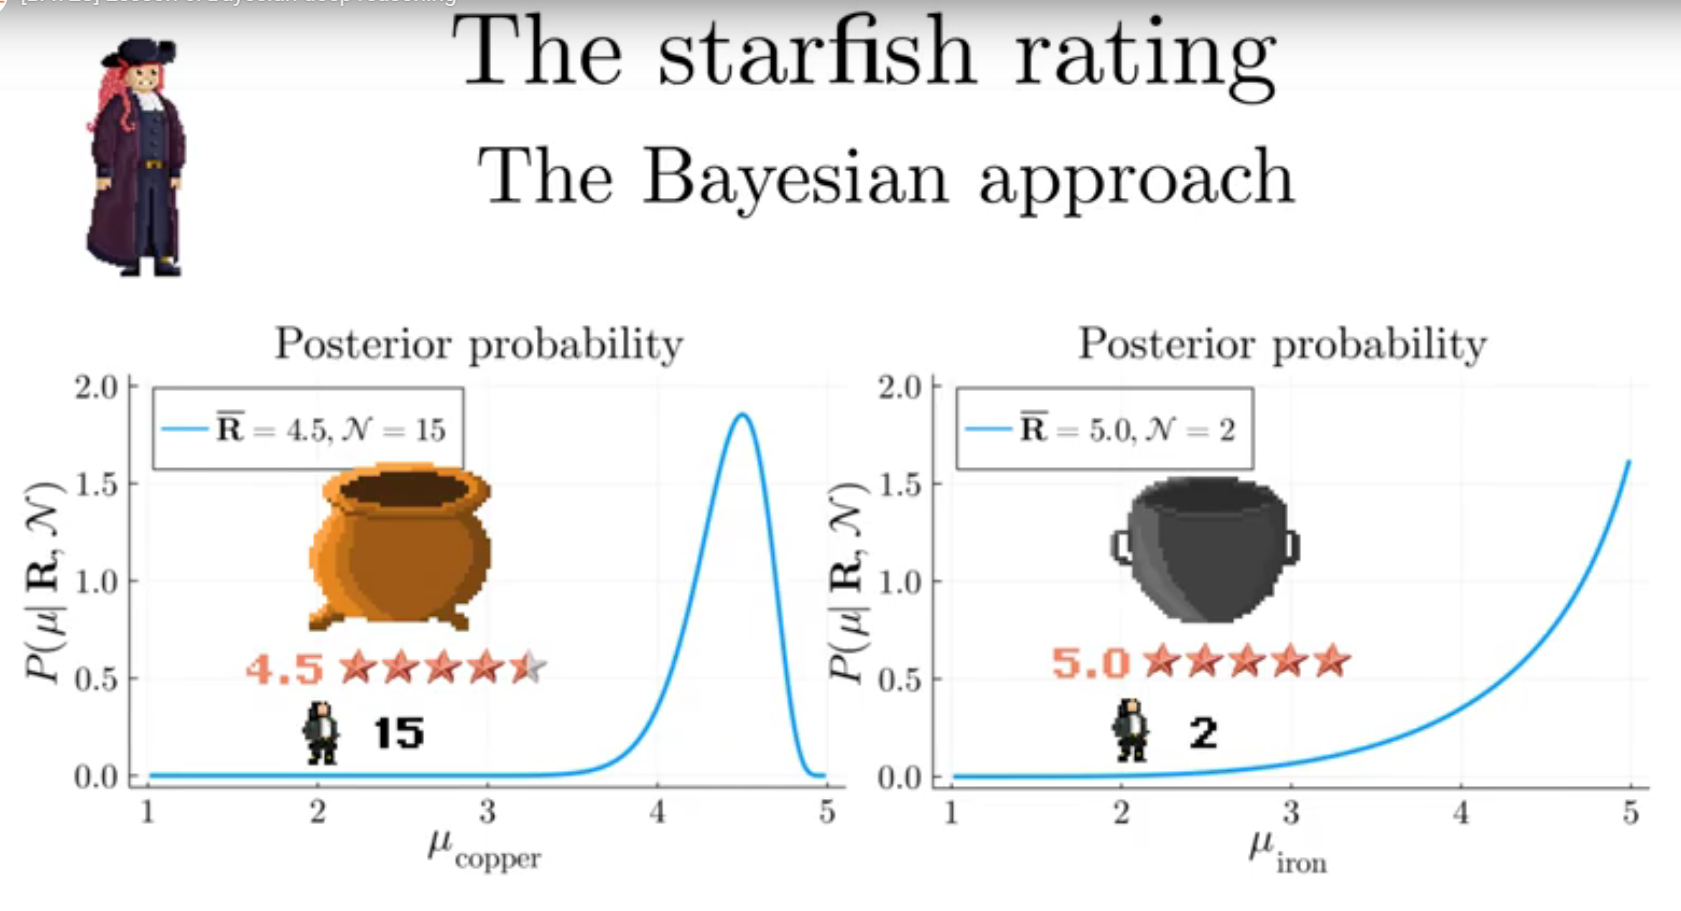
\includegraphics[width=0.75\textwidth]{6_11.png}
\end{figure}
We see
that the distribution of iron is much broader, as it is based on only 2 votes. We
have used an \textit{uninformative uniform prior}.
We can characterize the results by \textbf{mean $\pm$ standard deviation} and
obtain \[\bar{R}=4.5\rightarrow \mu_{copper}=4.4\pm0.2\qquad \bar{R}=5\rightarrow \mu_{iron}=4.4\pm0.5\]
This quantifies the observation of the previous statistical experiment that
the voting of the iron vessel is not very reliable and the iron vessel is not
really more popular than the tin pot.\\%6_12
 \begin{figure}[H]
	\centering
	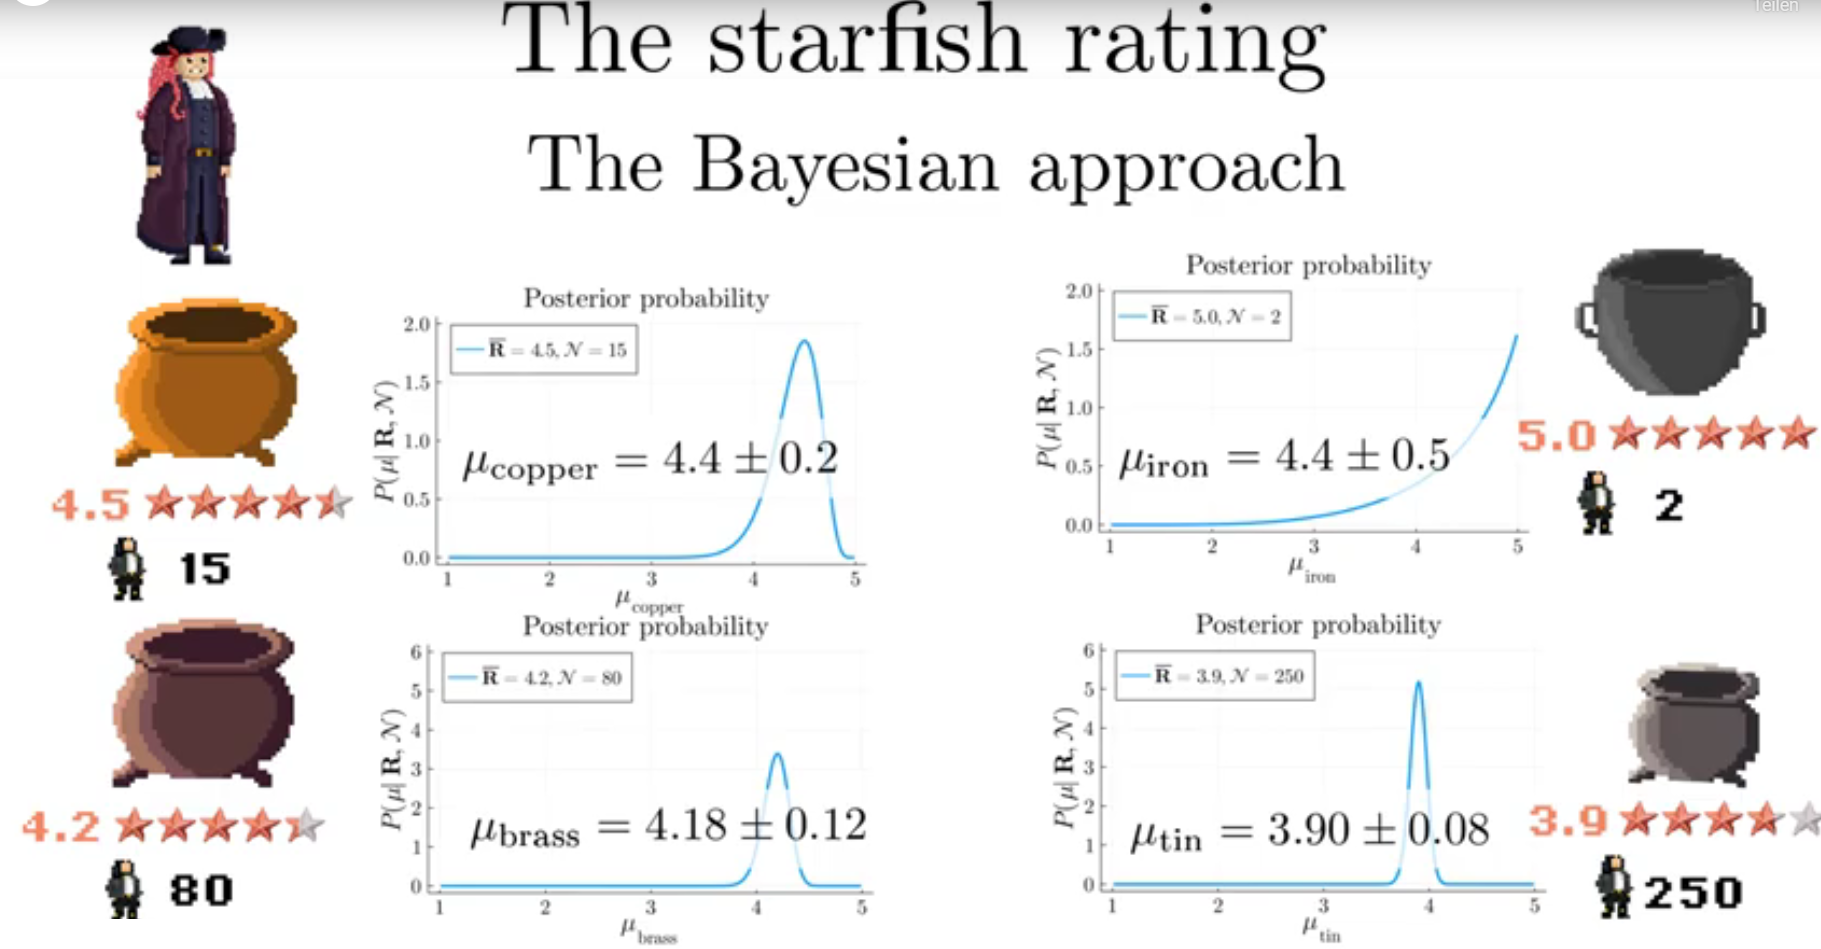
\includegraphics[width=0.75\textwidth]{6_12.png}
\end{figure}


Bayes’ theorem cannot only be used for inverse problems, it can also be considered 
as \textbf{update rule} for additional information.
Assume we have two independent data sets $D_1$ and $D_2$ and we want to infer
some parameters or answer any other question, which we will generically
denote as proposition $X$. By the definition of the conditional probability
and the product rule we obtain a remarkable formula.

\begin{equation*}\boxed{P(X|N_1,D_2)=\frac{P(X,D_1,D_2)}{P(D_1,D_2)}=\frac{P(D_2|X)P(X|D_1)}{P(D_2)}
}\end{equation*}\\

So instead of taking both data sets in one step into account, we can use it
iteratively. %6_13
 \begin{figure}[H]
	\centering
	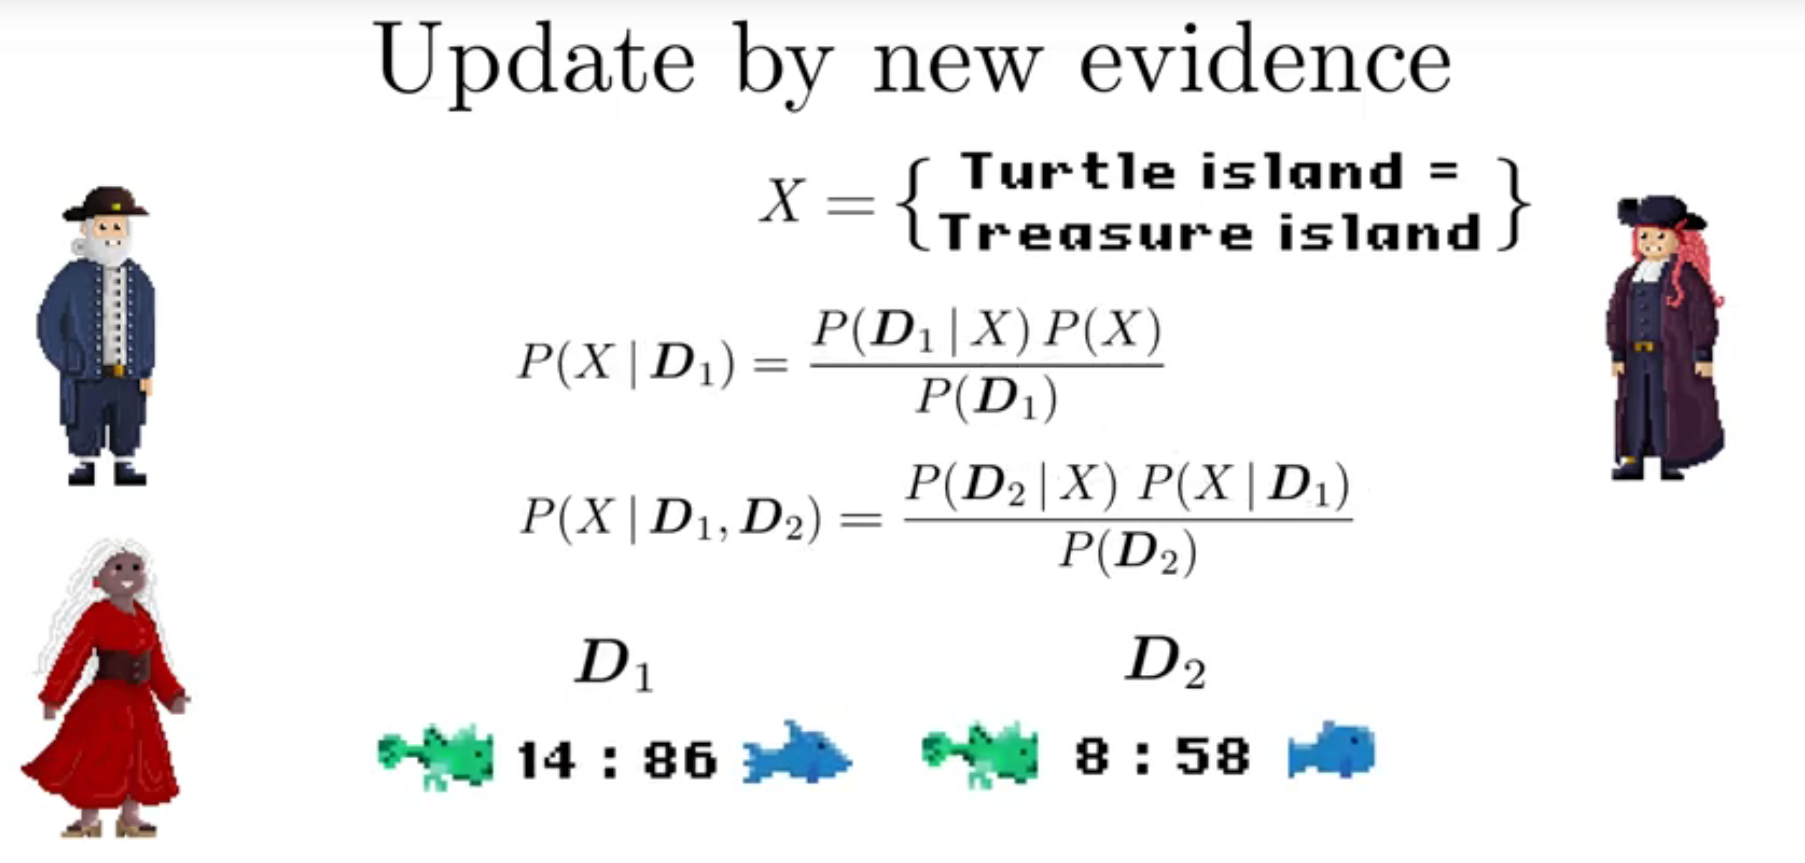
\includegraphics[width=0.75\textwidth]{6_13.png}
\end{figure}
In that case, $D_1$ defines the \textit{prior} $P(X|D_1)$ for the next iteration step, where $D_2$ is
taken into account.
The result of the posterior can again be summarized by the \textit{mode or maximum of
the posterior} which is called the \textbf{MAP} or the\textit{ mean to gain an estimation for the parameter
set X}.
The more reliable and robust estimator for the parameters is given by the \textbf{mean}.
This allows also to \textit{quantify its uncertainty} by the corresponding standard
deviation.%6_14
 \begin{figure}[H]
	\centering
	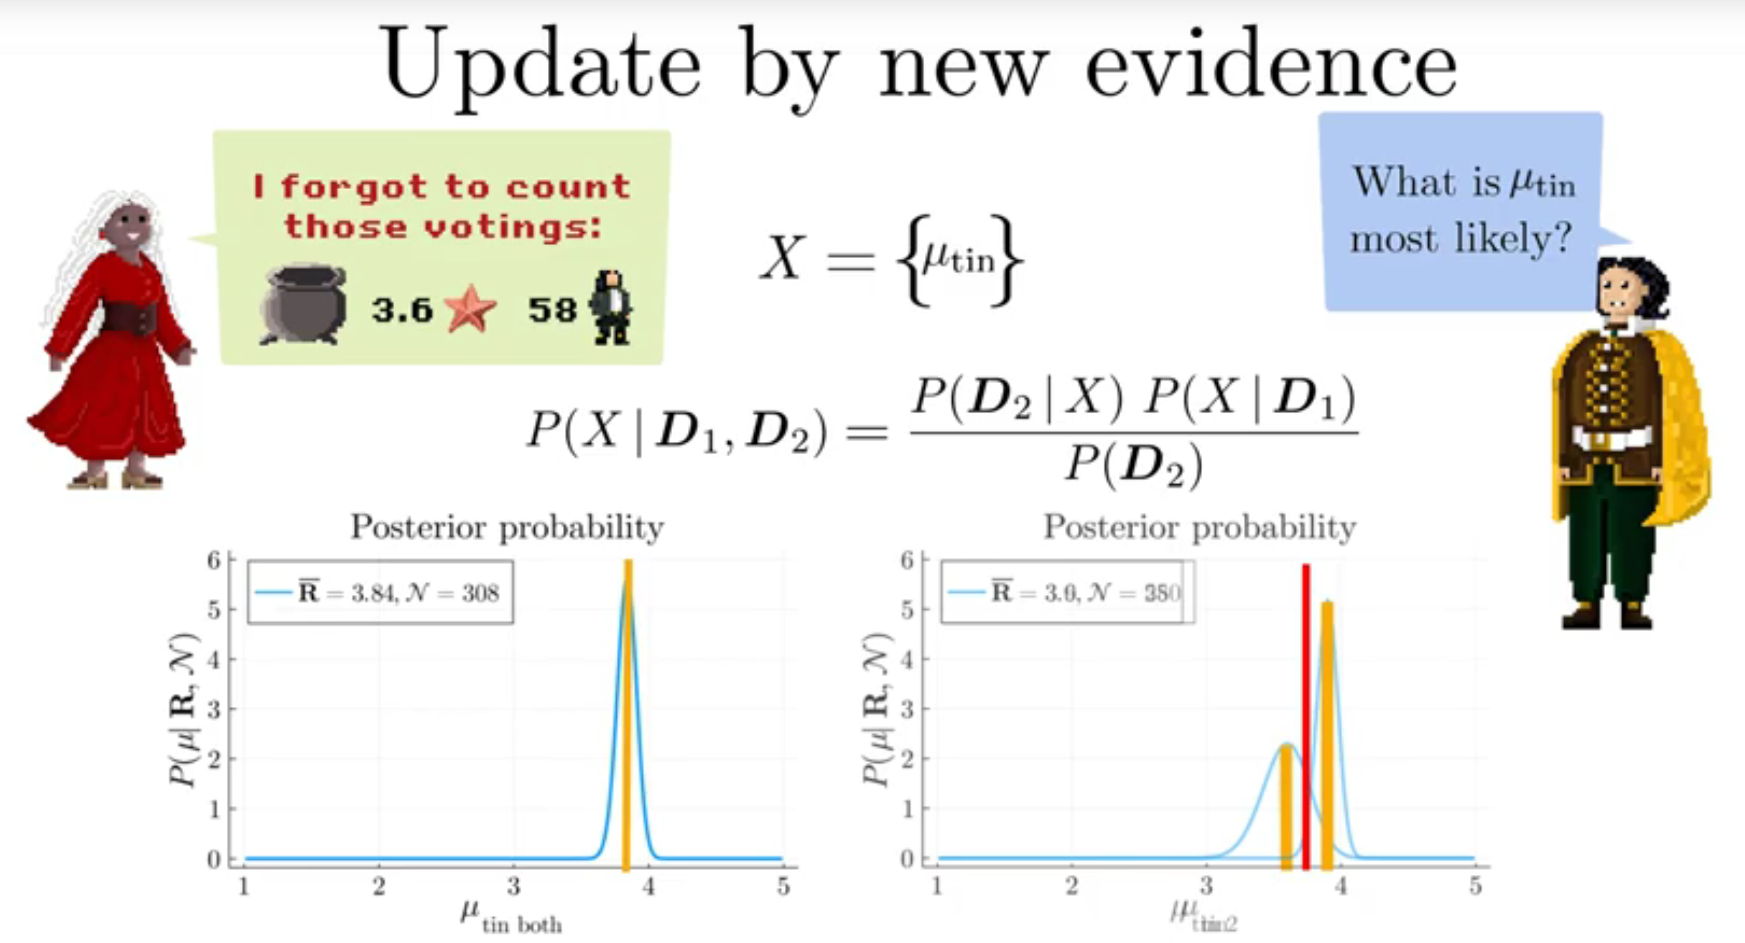
\includegraphics[width=0.75\textwidth]{6_14.png}
\end{figure}
Studying Bayes’ theorem and especially the relation of its parts in more detail
reveals many findings:\\%

\fbox{\parbox{\linewidth}{\textit{If the prior is constant then the posterior is proportional to the likelihood 
and the MAP solution is equal to what is called the \textbf{Maximum-Likelihood solution}.}}}\\

If the likelihood is Gaussian then Maximum-Likelihood is the same as
the standard \textbf{least squares approach}. We leave it up to you to proof
this statement.\\%

So far the \textbf{normalization} was a mere nuisance, but it actually has deeper
meaning. Suppose B encodes the measured data, for instance the positions of
Captain Bayes’ ship on the ocean measured at consecutive days, and $A_n$
describes exclusive and complete propositions about how these positions are
aligned. Say the positions are on a straight line, on a parabola, or completely
random. Then the probability for B is what is called the \textbf{data evidence} which is the
\textit{probability to find the measured data if these assumptions are correct}.\\


This concludes unit six. We have learned Bayes theorem and how to apply
it to inverse problems such as parameter estimation, model selection - think of 
treasure island - or hypothesis testing, which in the Bayesian frame is one
and the same thing.
We learned how to update probabilities based on new information and how
to assign prior probabilities using the maximum entropy principle.
Now it’s your turn to study more inverse problems in the bonus material and
to have a look at the interactive Pluto notebooks.
Please feel free to ask questions in the forum and feel encouraged to test your
knowledge in the quiz!

\end{document}